% !TeX root = main.tex
\section{研究范围与分析框架}\label{sec:framework}

\subsection{研究范围}\label{sec:framework-scope}

本文讨论偏好已作为输入给定的多目标序贯决策问题。这里的给定偏好可以是固定权重、非线性效用、目标优先关系或可接受性要求；而环境模型是否已知，则是与偏好无关的另一项信息条件。本文不讨论如何从比较反馈或示范中识别未知偏好，也不把一般静态多目标优化方法当作序贯问题的求解方法；静态标量化函数和解集指标只在用于构造长期准则或评价策略时讨论。

\subsection{基本模型}\label{sec:framework-model}

多目标 Markov 决策过程（MOMDP）是基本的建模形式。系统处于状态 $S_t$ 时选择动作 $A_t$，随后产生下一状态 $S_{t+1}$ 和多维回报 $\mathbf R_t\in\mathbb R^m$，其中 $m$ 为目标数。在完全观测且具有 Markov 性的情形下，下一状态和回报的条件分布由当前状态与动作决定；给定初始状态分布 $\rho_0$、评价时域及时间聚合规则后，策略决定了长期结果的分布\cite{roijers2013}。这一框架不要求模型能被求解器直接调用；状态只能部分观测时，策略要依据可用观测或信念状态做决策。

设 $h_t$ 为截至时刻 $t$ 决策者可获得的信息，策略一般写为 $\pi_t(a\mid h_t)$。相对于环境状态的 Markov 策略只依赖当前状态，历史依赖策略还可以利用累计回报、剩余预算等信息；是否允许动作随机化、时间依赖和记忆，都属于策略集合 $\Pi$ 的定义。对于有限时域折扣累计回报，记
\begin{equation}
\mathbf G^\pi=\sum_{t=0}^{T-1}\gamma^t\mathbf R_t,
\end{equation}
下文用小写 $\mathbf r_t$ 表示 $\mathbf R_t$ 的实现值。给定偏好 $p$ 后，需要规定如何评价这一随机向量或其他轨迹结果，再在允许的策略集合内比较策略。期望回报向量、完整结果分布和路径事件保留的信息各不相同，在评价准则确定之前不能相互替代\cite{hayes2022}。

图~\ref{fig:problem-overview}~展示了策略执行如何产生多维结果，以及给定偏好如何参与长期准则的定义。

\begin{figure}[H]
\centering
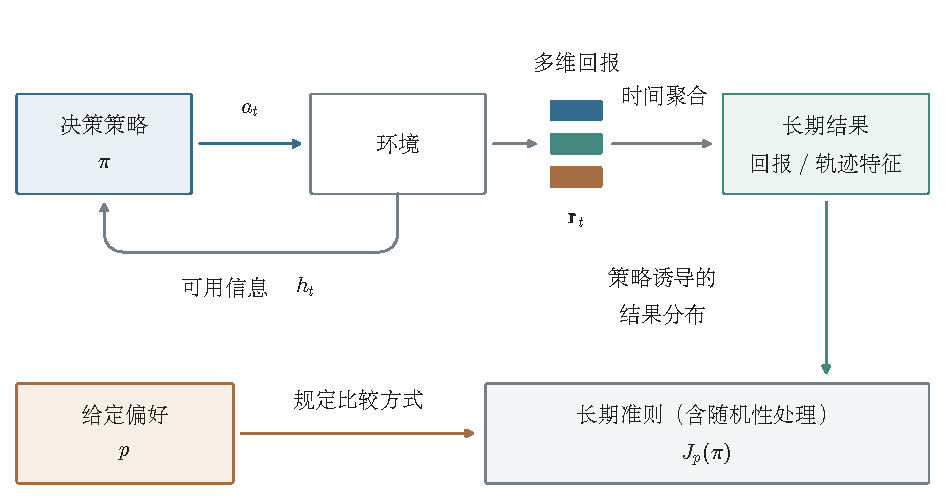
\includegraphics{figures/problem_overview.pdf}
\caption{给定偏好下的多目标序贯决策问题。策略依据可用信息 $h_t$ 选择动作 $a_t$，环境产生多维回报 $\mathbf r_t$，时间聚合形成长期结果。给定偏好、时间聚合与随机性处理共同规定策略比较准则 $J_p(\pi)$；图中的回路描述策略执行，不限定训练时的模型与数据来源\cite{hayes2022}。}
\label{fig:problem-overview}
\end{figure}

\subsection{分析框架}\label{sec:framework-dimensions}

围绕上述模型，本文从四个维度分析给定偏好下的多目标序贯决策问题。

\begin{enumerate}
\item \textbf{长期准则}：偏好以什么形式表达，作用于阶段结果、累计结果还是轨迹特征，跨阶段如何聚合，随机结果如何评价。这四项共同决定策略之间如何比较、哪些策略可以接受，由第~\ref{sec:criteria}~章展开。
\item \textbf{信息表示}：为了按长期准则比较策略，决策时必须保留哪些历史信息，价值函数要概括未来结果的哪些信息，以及这些表示是否支持递推求解。这部分在第~\ref{sec:structure-decomp}~至~\ref{sec:structure-recursion}~节讨论。
\item \textbf{策略类别}：最优解是否需要随机化、记忆或时间依赖，实际部署允许哪一类策略。策略类别问题在第~\ref{sec:structure-policy}~节处理。
\item \textbf{模型与数据条件}：环境模型是否可用、能否新增交互、历史数据记录了什么并覆盖了哪些区域。它决定前三个维度所需的信息从哪里获得，第~\ref{sec:solving}~章按这一维度组织求解方法。
\end{enumerate}

这四个维度并非并列，而是有先后关系：长期准则决定需要保留哪些信息；信息表示和策略类别限定了可搜索的决策规则；模型与数据条件则决定这些信息能否获得、以什么代价获得。第~\ref{sec:evaluation}~章的策略评价则回到第一个维度，检验求得的策略是否实现了原准则，评价所需的信息同样受第四个维度的限制。


这一框架也给出了比较不同方法的前提。两种方法只有在长期准则（包括初始状态分布和偏好语义）、策略类别和可用信息都一致时，性能差别才能归因于求解方法本身；任何一项不同，差别都可能来自问题设定。跨偏好的策略库和条件策略在本框架中被视为复用计算与数据的手段，其质量最终要落实到每个给定偏好下实际选出的策略上（第~\ref{sec:solving-reuse}~节和第~\ref{sec:eval-sets}~节）。
